\documentclass{article}

\usepackage{geometry}
\geometry{a4paper,margin=1in,}

\usepackage{hyperref}
\usepackage{graphicx}
\usepackage{float}
\usepackage{xcolor}

\definecolor{ag}{RGB}{112,173,71}
\definecolor{bl}{RGB}{196,89,18}
\definecolor{ds}{RGB}{255,0,0}
\definecolor{gw}{RGB}{255,191,4}
\definecolor{lw}{RGB}{112,48,160}

\title{COSC345 App Proposal}

%Names in alphabetical order by surname
\author{Burnie Lorimer (2367465) Damian Soo (6551336) \\ Garth Wales (4861462) Louis Whitburn (2548261)}
\date{\today}

\begin{document}
	\maketitle
	
	\section{What we intend to build}
	
	We are building an android app to display university course material. This will be targeted towards displaying content from \url{cs.otago.ac.nz} primarily. It will provide an easy to view format of each paper for mobile devices. Information will be pulled from the websites themselves and formatted.
	
	\subsection{Requirements}
	
	\begin{itemize}
		\item Should support differentiating between lecture, tutorial and assignment PDFs for undergraduate COSC papers, and handle PDFs in general for undergraduate MATH/STAT papers.
		\item Should support querying marks for undergraduate COSC and undergraduate MATH/STAT papers.
		\item Should be able to download and display a PDF file to the user within 3s of the user selecting it.
		\item Should be able to display a downloaded (i.e. cached) PDF within 0.5s of the user selecting it.
		\item Should warn the user before downloading on mobile data.
	\end{itemize}
	
	A stretch goal is to include postgraduate papers COSC, MATH and STAT papers. This could be implemented if we run ahead of schedule.
	
	\section{Our anarchists \textit{(and their expertise)}} 
	
	Our team consists of: 
	\begin{itemize}
		\item Burnie Lorimer - Programming (Webpage parsing)
		\item Damian Soo – Programming (General)
		\item Garth Wales – UI development
		\item Louis Whitburn – Programming (Storage/General)
	\end{itemize}

	\section{How we are going to build it}

	We will use Android Studio with Kotlin, We intend to target Android API level 29 (Android version 10). The app will function by using common formats of each department to guess the locations of papers lecture slides or other information. An example being \url{cs.otago.ac.nz/(papercode)/lectures.php} is where most COSC papers have their lecture slide PDFs. The app will then cache and display the information from these pages.

	\section{How long it will take to build}

	We will begin by implementing PDF viewing capabilities and pulling the PDF from one specific paper, then expand into a better dynamic system. 

	It will take roughly 5 months of part time work to complete the app, including some time for unexpected issues or setbacks.
	
	The key targets and milestones are laid out below.
	
	\begin{itemize}
		\item Whole group: {\color{ag} \rule{\baselineskip}{\baselineskip}}
		\item Burnie Lorimer: {\color{bl} \rule{\baselineskip}{\baselineskip}}
		\item Damian Soo: {\color{ds} \rule{\baselineskip}{\baselineskip}}
		\item Garth Wales: {\color{gw} \rule{\baselineskip}{\baselineskip}}
		\item Louis Whitburn: {\color{lw} \rule{\baselineskip}{\baselineskip}}
	\end{itemize}
	
	\begin{figure}[H]
		\centering
		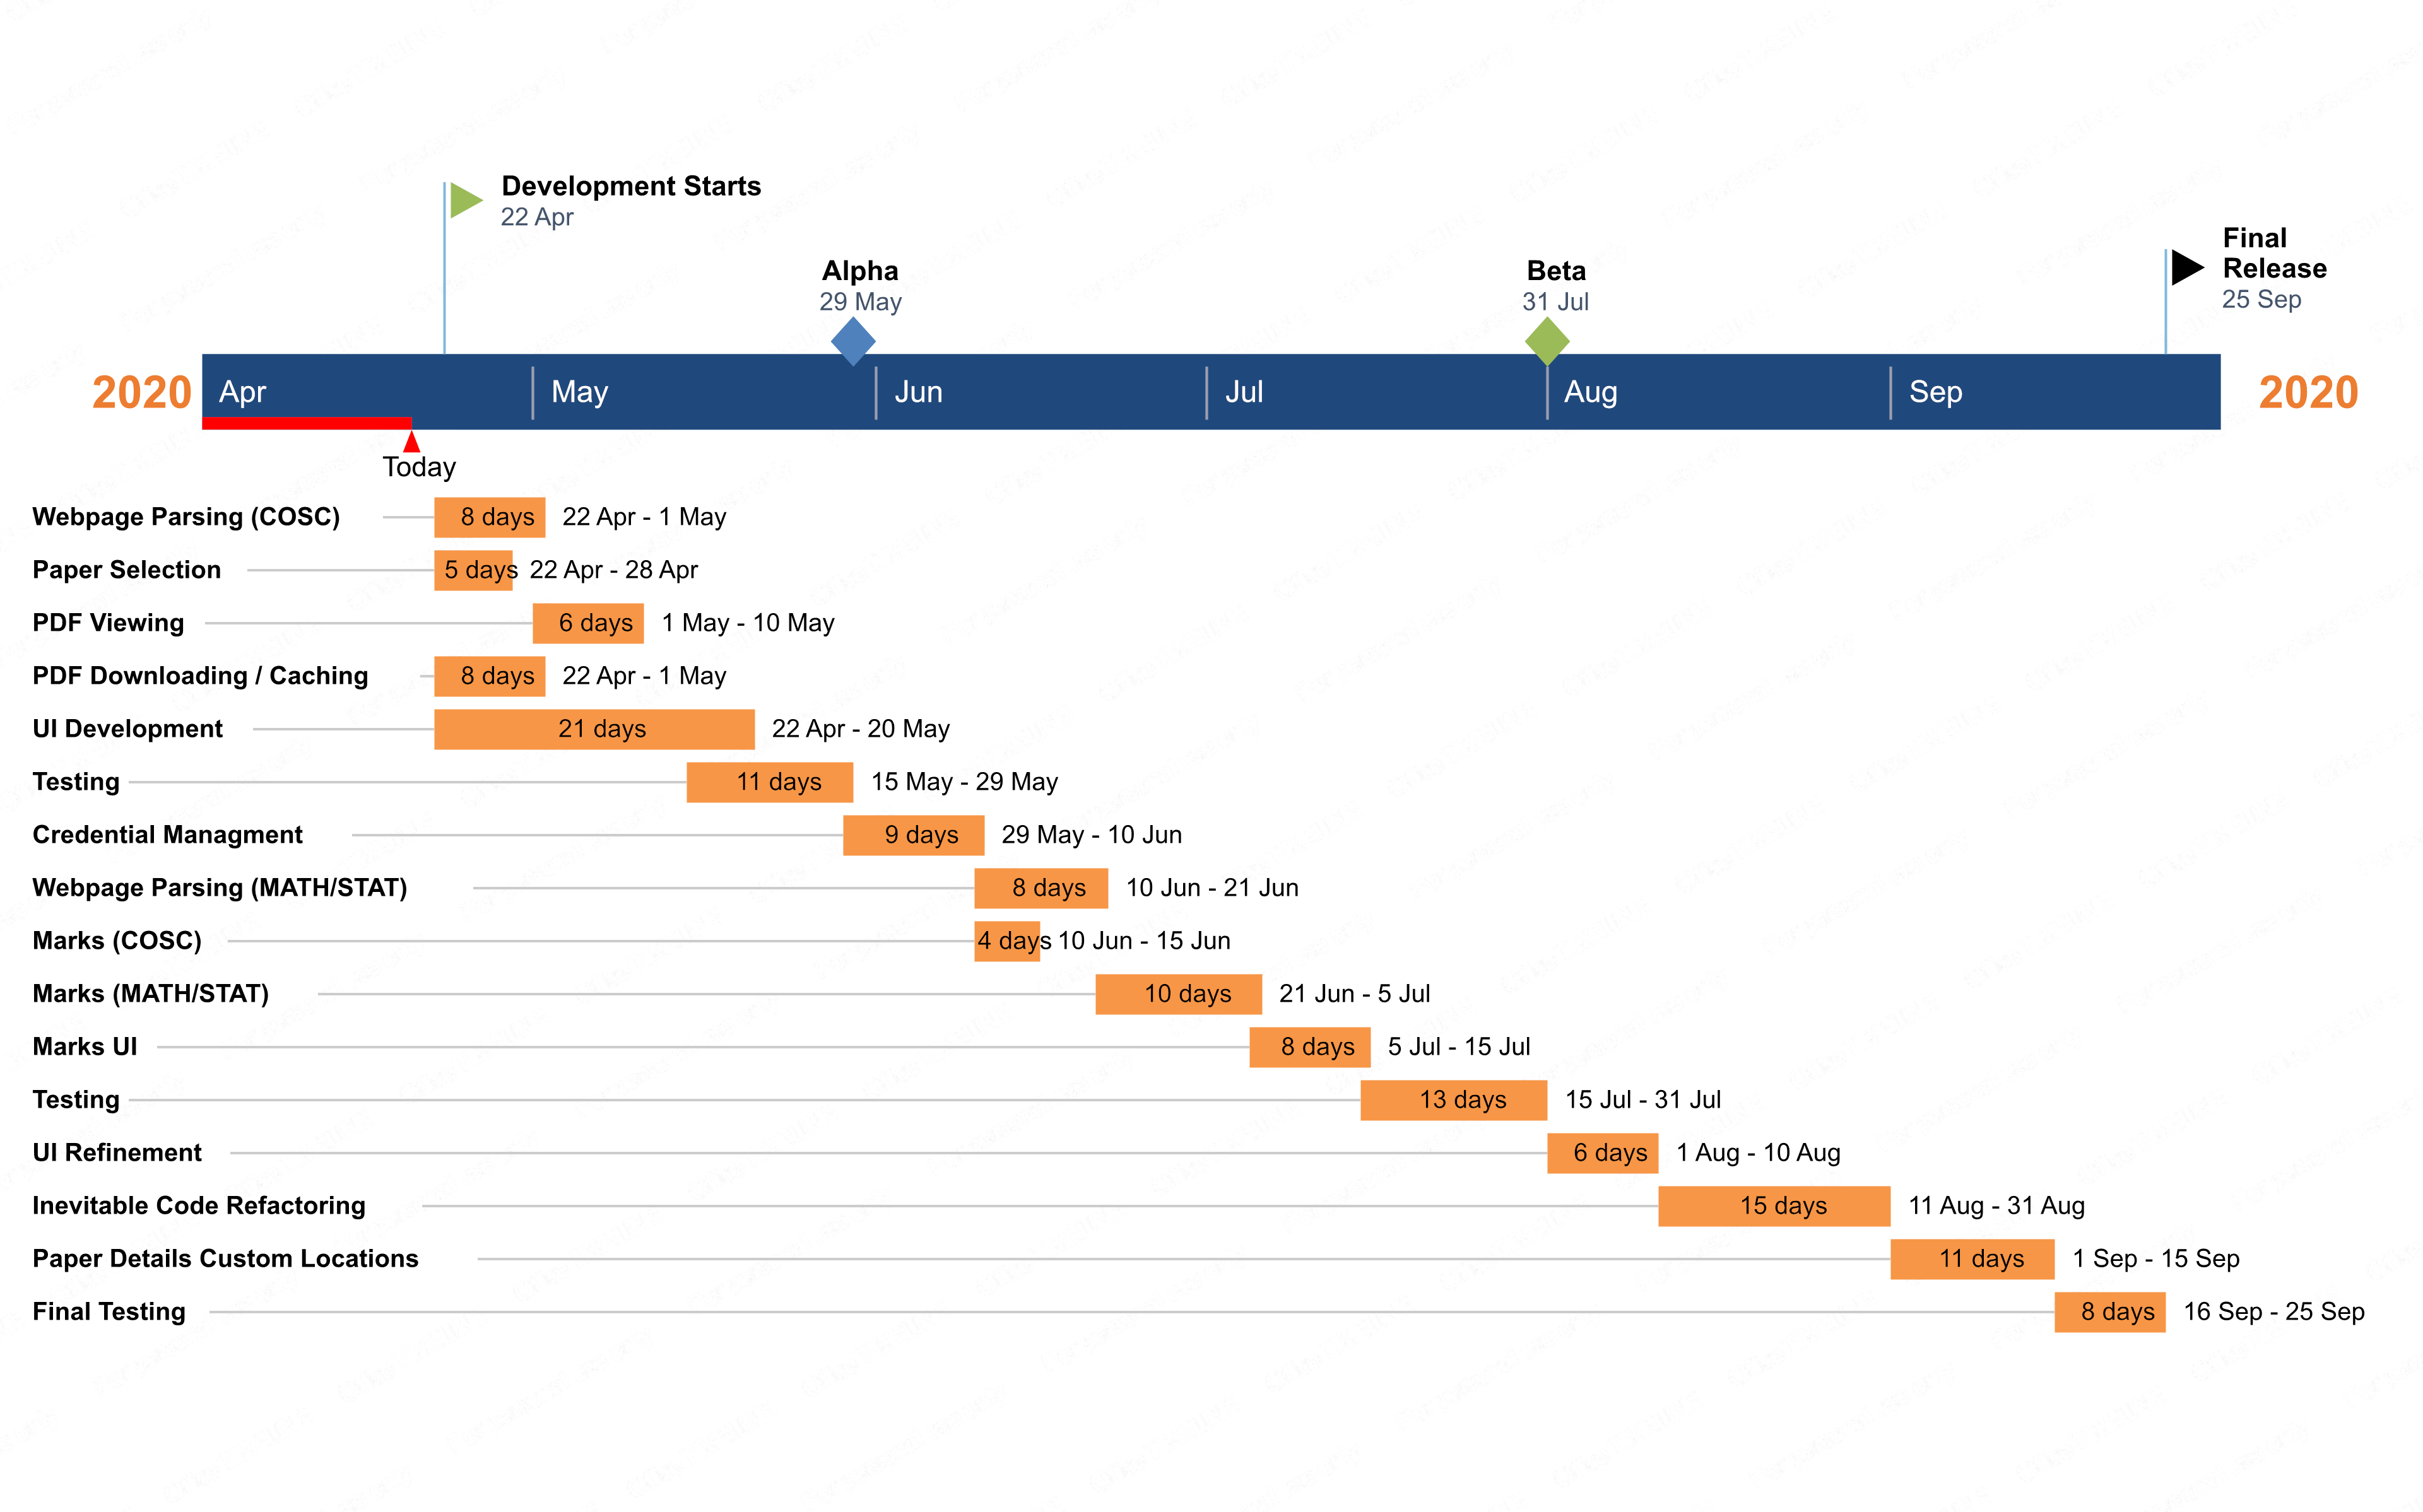
\includegraphics[width=\linewidth]{chart.png}
	\end{figure}
	
	\section{Pre-existing options and causing irritation}
	
	The establishment already has websites such as \url{cs.otago.ac.nz}. However, these websites are rubbish on mobile devices and they do not provide any mobile solutions. We will irritate the establishment by creating a better alternative to their existing solutions. We will be doing this with our source code hosted on the establishment's own GitLab server \url{altitude.otago.ac.nz} to add insult to injury.
	
	We also considered some other options for causing anarchy, but discounted them due to potential legal issues:
	
	\begin{enumerate}
		\item Emailing the lecturers statistics of which students have looked at which lectures.
		\item Parsing PDFs for assignment due dates and preventing use of our app on such dates (and the previous day as well). Use of the app on such days could be unlocked for a nominal fee.
	\end{enumerate}
	
	\section{Risks}
	
	Our biggest risk is website formats changing causing the app to no longer function. Either with individual papers changing the layout or using different systems such as blackboard. For blackboard and the MATH/STAT pages we will explore credential storage to access pages behind passwords to ensure we have full coverage. A workaround for this is allowing users to specify custom locations for resources.
	
	The next largest risk is not meeting deliverables / milestones. This is easily mitigated by simply sticking to the above chart\footnote{If every project just stuck to schedule then we would live in a world in which software was always delivered on time and bug free. Since this is not the world we live in it is reasonable to assume that that advice is rather unhelpful. However in a university environment stating the obvious about deadlines is not without merit.}. In addition assignments of tasks to people may be shifted around as needed, and we will ``meet''\footnote{In some capacity} weekly.
	
	Other risks include unfamiliarity with Kotlin and Android development, and the volatile COVID-19 situation (although other illnesses are more likely).
\end{document}
